% Created by tikzDevice version 0.11 on 2018-04-11 18:30:51
% !TEX encoding = UTF-8 Unicode
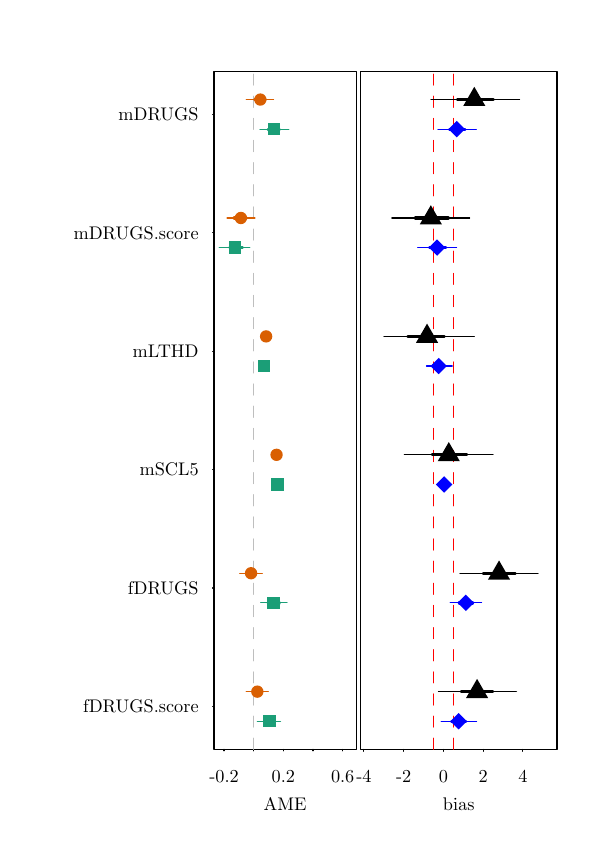
\begin{tikzpicture}[x=1pt,y=1pt]
\definecolor{fillColor}{RGB}{255,255,255}
\path[use as bounding box,fill=fillColor,fill opacity=0.00] (0,0) rectangle (199.17,284.53);
\begin{scope}
\path[clip] (  0.00,  0.00) rectangle (199.17,284.53);
\definecolor{drawColor}{RGB}{0,0,0}

\path[draw=drawColor,line width= 0.4pt,line join=round,line cap=round] ( 70.94, 23.76) -- (113.83, 23.76);

\path[draw=drawColor,line width= 0.4pt,line join=round,line cap=round] ( 70.94, 23.76) -- ( 70.94, 23.25);

\path[draw=drawColor,line width= 0.4pt,line join=round,line cap=round] ( 81.67, 23.76) -- ( 81.67, 23.25);

\path[draw=drawColor,line width= 0.4pt,line join=round,line cap=round] ( 92.39, 23.76) -- ( 92.39, 23.25);

\path[draw=drawColor,line width= 0.4pt,line join=round,line cap=round] (103.11, 23.76) -- (103.11, 23.25);

\path[draw=drawColor,line width= 0.4pt,line join=round,line cap=round] (113.83, 23.76) -- (113.83, 23.25);

\node[text=drawColor,anchor=base,inner sep=0pt, outer sep=0pt, scale=  0.66] at ( 70.94, 11.88) {-0.2};

\node[text=drawColor,anchor=base,inner sep=0pt, outer sep=0pt, scale=  0.66] at ( 92.39, 11.88) {0.2};

\node[text=drawColor,anchor=base,inner sep=0pt, outer sep=0pt, scale=  0.66] at (113.83, 11.88) {0.6};

\path[draw=drawColor,line width= 0.4pt,line join=round,line cap=round] ( 67.32, 23.76) --
	(118.71, 23.76) --
	(118.71,268.69) --
	( 67.32,268.69) --
	( 67.32, 23.76);
\end{scope}
\begin{scope}
\path[clip] (  0.00,  0.00) rectangle (119.50,284.53);
\definecolor{drawColor}{RGB}{0,0,0}

\node[text=drawColor,anchor=base,inner sep=0pt, outer sep=0pt, scale=  0.66] at ( 93.01,  1.58) {AME};
\end{scope}
\begin{scope}
\path[clip] ( 67.32, 23.76) rectangle (118.71,268.69);
\definecolor{drawColor}{RGB}{190,190,190}

\path[draw=drawColor,line width= 0.4pt,dash pattern=on 4pt off 4pt ,line join=round,line cap=round] ( 81.67, 23.76) -- ( 81.67,268.69);
\definecolor{fillColor}{RGB}{27,158,119}

\path[fill=fillColor] ( 86.78,245.62) --
	( 91.24,245.62) --
	( 91.24,250.08) --
	( 86.78,250.08) --
	cycle;

\path[fill=fillColor] ( 72.68,202.83) --
	( 77.13,202.83) --
	( 77.13,207.29) --
	( 72.68,207.29) --
	cycle;

\path[fill=fillColor] ( 83.08,160.04) --
	( 87.53,160.04) --
	( 87.53,164.50) --
	( 83.08,164.50) --
	cycle;

\path[fill=fillColor] ( 88.03,117.25) --
	( 92.49,117.25) --
	( 92.49,121.71) --
	( 88.03,121.71) --
	cycle;

\path[fill=fillColor] ( 86.62, 74.46) --
	( 91.07, 74.46) --
	( 91.07, 78.92) --
	( 86.62, 78.92) --
	cycle;

\path[fill=fillColor] ( 85.12, 31.67) --
	( 89.58, 31.67) --
	( 89.58, 36.13) --
	( 85.12, 36.13) --
	cycle;
\definecolor{drawColor}{RGB}{27,158,119}

\path[draw=drawColor,line width= 1.2pt,line join=round,line cap=round] ( 86.80,247.85) -- ( 91.00,247.85);

\path[draw=drawColor,line width= 1.2pt,line join=round,line cap=round] ( 72.96,205.06) -- ( 77.65,205.06);

\path[draw=drawColor,line width= 1.2pt,line join=round,line cap=round] ( 84.61,162.27) -- ( 86.00,162.27);

\path[draw=drawColor,line width= 1.2pt,line join=round,line cap=round] ( 89.68,119.48) -- ( 91.24,119.48);

\path[draw=drawColor,line width= 1.2pt,line join=round,line cap=round] ( 86.99, 76.69) -- ( 90.84, 76.69);

\path[draw=drawColor,line width= 1.2pt,line join=round,line cap=round] ( 85.55, 33.90) -- ( 89.13, 33.90);

\path[draw=drawColor,line width= 0.4pt,line join=round,line cap=round] ( 83.91,247.85) -- ( 94.35,247.85);

\path[draw=drawColor,line width= 0.4pt,line join=round,line cap=round] ( 69.22,205.06) -- ( 80.27,205.06);

\path[draw=drawColor,line width= 0.4pt,line join=round,line cap=round] ( 83.62,162.27) -- ( 87.00,162.27);

\path[draw=drawColor,line width= 0.4pt,line join=round,line cap=round] ( 88.35,119.48) -- ( 92.26,119.48);

\path[draw=drawColor,line width= 0.4pt,line join=round,line cap=round] ( 84.21, 76.69) -- ( 93.72, 76.69);

\path[draw=drawColor,line width= 0.4pt,line join=round,line cap=round] ( 82.97, 33.90) -- ( 91.35, 33.90);
\definecolor{fillColor}{RGB}{217,95,2}

\path[fill=fillColor] ( 84.07,258.55) circle (  2.23);

\path[fill=fillColor] ( 77.04,215.76) circle (  2.23);

\path[fill=fillColor] ( 86.16,172.97) circle (  2.23);

\path[fill=fillColor] ( 89.93,130.18) circle (  2.23);

\path[fill=fillColor] ( 80.72, 87.39) circle (  2.23);

\path[fill=fillColor] ( 82.98, 44.60) circle (  2.23);
\definecolor{drawColor}{RGB}{217,95,2}

\path[draw=drawColor,line width= 1.2pt,line join=round,line cap=round] ( 81.94,258.55) -- ( 85.98,258.55);

\path[draw=drawColor,line width= 1.2pt,line join=round,line cap=round] ( 74.70,215.76) -- ( 78.85,215.76);

\path[draw=drawColor,line width= 1.2pt,line join=round,line cap=round] ( 85.52,172.97) -- ( 86.86,172.97);

\path[draw=drawColor,line width= 1.2pt,line join=round,line cap=round] ( 89.13,130.18) -- ( 90.51,130.18);

\path[draw=drawColor,line width= 1.2pt,line join=round,line cap=round] ( 79.15, 87.39) -- ( 82.56, 87.39);

\path[draw=drawColor,line width= 1.2pt,line join=round,line cap=round] ( 81.27, 44.60) -- ( 84.58, 44.60);

\path[draw=drawColor,line width= 0.4pt,line join=round,line cap=round] ( 78.99,258.55) -- ( 88.89,258.55);

\path[draw=drawColor,line width= 0.4pt,line join=round,line cap=round] ( 72.04,215.76) -- ( 82.13,215.76);

\path[draw=drawColor,line width= 0.4pt,line join=round,line cap=round] ( 84.47,172.97) -- ( 87.75,172.97);

\path[draw=drawColor,line width= 0.4pt,line join=round,line cap=round] ( 88.24,130.18) -- ( 91.64,130.18);

\path[draw=drawColor,line width= 0.4pt,line join=round,line cap=round] ( 76.62, 87.39) -- ( 84.81, 87.39);

\path[draw=drawColor,line width= 0.4pt,line join=round,line cap=round] ( 78.97, 44.60) -- ( 86.99, 44.60);
\end{scope}
\begin{scope}
\path[clip] (  0.00,  0.00) rectangle (199.17,284.53);
\definecolor{drawColor}{RGB}{0,0,0}

\path[draw=drawColor,line width= 0.4pt,line join=round,line cap=round] ( 67.32, 39.25) -- ( 67.32,253.20);

\path[draw=drawColor,line width= 0.4pt,line join=round,line cap=round] ( 67.32, 39.25) -- ( 66.81, 39.25);

\path[draw=drawColor,line width= 0.4pt,line join=round,line cap=round] ( 67.32, 82.04) -- ( 66.81, 82.04);

\path[draw=drawColor,line width= 0.4pt,line join=round,line cap=round] ( 67.32,124.83) -- ( 66.81,124.83);

\path[draw=drawColor,line width= 0.4pt,line join=round,line cap=round] ( 67.32,167.62) -- ( 66.81,167.62);

\path[draw=drawColor,line width= 0.4pt,line join=round,line cap=round] ( 67.32,210.41) -- ( 66.81,210.41);

\path[draw=drawColor,line width= 0.4pt,line join=round,line cap=round] ( 67.32,253.20) -- ( 66.81,253.20);

\node[text=drawColor,anchor=base east,inner sep=0pt, outer sep=0pt, scale=  0.66] at ( 61.78, 36.98) {fDRUGS.score};

\node[text=drawColor,anchor=base east,inner sep=0pt, outer sep=0pt, scale=  0.66] at ( 61.78, 79.77) {fDRUGS};

\node[text=drawColor,anchor=base east,inner sep=0pt, outer sep=0pt, scale=  0.66] at ( 61.78,122.56) {mSCL5};

\node[text=drawColor,anchor=base east,inner sep=0pt, outer sep=0pt, scale=  0.66] at ( 61.78,165.35) {mLTHD};

\node[text=drawColor,anchor=base east,inner sep=0pt, outer sep=0pt, scale=  0.66] at ( 61.78,208.14) {mDRUGS.score};

\node[text=drawColor,anchor=base east,inner sep=0pt, outer sep=0pt, scale=  0.66] at ( 61.78,250.92) {mDRUGS};
\end{scope}
\begin{scope}
\path[clip] ( 67.32, 23.76) rectangle (118.71,268.69);
\definecolor{drawColor}{RGB}{0,0,0}

\path[draw=drawColor,line width= 0.4pt,line join=round,line cap=round] ( 67.32,273.31) -- (118.71,273.31);

\path[draw=drawColor,line width= 0.4pt,line join=round,line cap=round] ( 67.32,275.88) -- (118.71,275.88);

\path[draw=drawColor,line width= 0.4pt,line join=round,line cap=round] ( 67.32, 16.57) -- (118.71, 16.57);

\path[draw=drawColor,line width= 0.4pt,line join=round,line cap=round] ( 67.32, 19.14) -- (118.71, 19.14);
\end{scope}
\begin{scope}
\path[clip] (  0.00,  0.00) rectangle (199.17,284.53);
\definecolor{drawColor}{RGB}{0,0,0}

\path[draw=drawColor,line width= 0.4pt,line join=round,line cap=round] (121.49, 23.76) -- (178.93, 23.76);

\path[draw=drawColor,line width= 0.4pt,line join=round,line cap=round] (121.49, 23.76) -- (121.49, 23.05);

\path[draw=drawColor,line width= 0.4pt,line join=round,line cap=round] (135.85, 23.76) -- (135.85, 23.05);

\path[draw=drawColor,line width= 0.4pt,line join=round,line cap=round] (150.21, 23.76) -- (150.21, 23.05);

\path[draw=drawColor,line width= 0.4pt,line join=round,line cap=round] (164.57, 23.76) -- (164.57, 23.05);

\path[draw=drawColor,line width= 0.4pt,line join=round,line cap=round] (178.93, 23.76) -- (178.93, 23.05);

\node[text=drawColor,anchor=base,inner sep=0pt, outer sep=0pt, scale=  0.66] at (121.49, 11.88) {-4};

\node[text=drawColor,anchor=base,inner sep=0pt, outer sep=0pt, scale=  0.66] at (135.85, 11.88) {-2};

\node[text=drawColor,anchor=base,inner sep=0pt, outer sep=0pt, scale=  0.66] at (150.21, 11.88) {0};

\node[text=drawColor,anchor=base,inner sep=0pt, outer sep=0pt, scale=  0.66] at (164.57, 11.88) {2};

\node[text=drawColor,anchor=base,inner sep=0pt, outer sep=0pt, scale=  0.66] at (178.93, 11.88) {4};

\path[draw=drawColor,line width= 0.4pt,line join=round,line cap=round] (120.29, 23.76) --
	(191.25, 23.76) --
	(191.25,268.69) --
	(120.29,268.69) --
	(120.29, 23.76);
\end{scope}
\begin{scope}
\path[clip] (119.50,  0.00) rectangle (199.17,284.53);
\definecolor{drawColor}{RGB}{0,0,0}

\node[text=drawColor,anchor=base,inner sep=0pt, outer sep=0pt, scale=  0.66] at (155.77,  1.58) {bias};
\end{scope}
\begin{scope}
\path[clip] (120.29, 23.76) rectangle (191.25,268.69);
\definecolor{drawColor}{RGB}{255,0,0}

\path[draw=drawColor,line width= 0.4pt,dash pattern=on 4pt off 4pt ,line join=round,line cap=round] (146.62, 23.76) -- (146.62,268.69);

\path[draw=drawColor,line width= 0.4pt,dash pattern=on 4pt off 4pt ,line join=round,line cap=round] (153.80, 23.76) -- (153.80,268.69);
\definecolor{drawColor}{RGB}{0,0,0}

\path[draw=drawColor,line width= 0.4pt,line join=round,line cap=round] (145.72,258.55) -- (177.72,258.55);

\path[draw=drawColor,line width= 0.4pt,line join=round,line cap=round] (131.59,215.76) -- (159.70,215.76);

\path[draw=drawColor,line width= 0.4pt,line join=round,line cap=round] (128.75,172.97) -- (161.40,172.97);

\path[draw=drawColor,line width= 0.4pt,line join=round,line cap=round] (136.09,130.18) -- (168.18,130.18);

\path[draw=drawColor,line width= 0.4pt,line join=round,line cap=round] (156.20, 87.39) -- (184.44, 87.39);

\path[draw=drawColor,line width= 0.4pt,line join=round,line cap=round] (148.44, 44.60) -- (176.62, 44.60);

\path[draw=drawColor,line width= 1.2pt,line join=round,line cap=round] (155.25,258.55) -- (168.30,258.55);

\path[draw=drawColor,line width= 1.2pt,line join=round,line cap=round] (140.15,215.76) -- (151.93,215.76);

\path[draw=drawColor,line width= 1.2pt,line join=round,line cap=round] (137.35,172.97) -- (150.58,172.97);

\path[draw=drawColor,line width= 1.2pt,line join=round,line cap=round] (146.13,130.18) -- (158.67,130.18);

\path[draw=drawColor,line width= 1.2pt,line join=round,line cap=round] (164.59, 87.39) -- (176.23, 87.39);

\path[draw=drawColor,line width= 1.2pt,line join=round,line cap=round] (156.63, 44.60) -- (168.06, 44.60);
\definecolor{drawColor}{RGB}{0,0,255}

\path[draw=drawColor,line width= 0.4pt,line join=round,line cap=round] (148.27,247.85) -- (162.09,247.85);

\path[draw=drawColor,line width= 0.4pt,line join=round,line cap=round] (140.90,205.06) -- (154.95,205.06);

\path[draw=drawColor,line width= 0.4pt,line join=round,line cap=round] (144.09,162.27) -- (153.40,162.27);

\path[draw=drawColor,line width= 0.4pt,line join=round,line cap=round] (148.22,119.48) -- (152.75,119.48);

\path[draw=drawColor,line width= 0.4pt,line join=round,line cap=round] (152.63, 76.69) -- (164.04, 76.69);

\path[draw=drawColor,line width= 0.4pt,line join=round,line cap=round] (149.41, 33.90) -- (162.19, 33.90);

\path[draw=drawColor,line width= 1.2pt,line join=round,line cap=round] (152.39,247.85) -- (158.02,247.85);

\path[draw=drawColor,line width= 1.2pt,line join=round,line cap=round] (145.18,205.06) -- (151.07,205.06);

\path[draw=drawColor,line width= 1.2pt,line join=round,line cap=round] (146.54,162.27) -- (150.32,162.27);

\path[draw=drawColor,line width= 1.2pt,line join=round,line cap=round] (149.63,119.48) -- (151.41,119.48);

\path[draw=drawColor,line width= 1.2pt,line join=round,line cap=round] (156.02, 76.69) -- (160.72, 76.69);

\path[draw=drawColor,line width= 1.2pt,line join=round,line cap=round] (153.12, 33.90) -- (158.30, 33.90);
\definecolor{fillColor}{RGB}{0,0,0}

\path[fill=fillColor] (161.39,263.17) --
	(165.39,256.24) --
	(157.39,256.24) --
	cycle;

\path[fill=fillColor] (145.68,220.38) --
	(149.68,213.45) --
	(141.68,213.45) --
	cycle;

\path[fill=fillColor] (144.31,177.59) --
	(148.31,170.66) --
	(140.32,170.66) --
	cycle;

\path[fill=fillColor] (152.17,134.80) --
	(156.17,127.87) --
	(148.17,127.87) --
	cycle;

\path[fill=fillColor] (170.33, 92.01) --
	(174.33, 85.08) --
	(166.33, 85.08) --
	cycle;

\path[fill=fillColor] (162.39, 49.22) --
	(166.39, 42.29) --
	(158.39, 42.29) --
	cycle;
\definecolor{fillColor}{RGB}{0,0,255}

\path[fill=fillColor] (152.07,247.85) --
	(155.04,250.82) --
	(158.01,247.85) --
	(155.04,244.88) --
	cycle;

\path[fill=fillColor] (144.97,205.06) --
	(147.94,208.03) --
	(150.91,205.06) --
	(147.94,202.09) --
	cycle;

\path[fill=fillColor] (145.56,162.27) --
	(148.53,165.24) --
	(151.50,162.27) --
	(148.53,159.30) --
	cycle;

\path[fill=fillColor] (147.52,119.48) --
	(150.49,122.45) --
	(153.46,119.48) --
	(150.49,116.51) --
	cycle;

\path[fill=fillColor] (155.37, 76.69) --
	(158.34, 79.66) --
	(161.31, 76.69) --
	(158.34, 73.72) --
	cycle;

\path[fill=fillColor] (152.76, 33.90) --
	(155.73, 36.87) --
	(158.70, 33.90) --
	(155.73, 30.93) --
	cycle;
\end{scope}
\begin{scope}
\path[clip] (120.29, 23.76) rectangle (191.25,268.69);
\definecolor{drawColor}{RGB}{0,0,0}

\path[draw=drawColor,line width= 0.4pt,line join=round,line cap=round] (120.29,273.31) -- (191.25,273.31);

\path[draw=drawColor,line width= 0.4pt,line join=round,line cap=round] (120.29,275.88) -- (191.25,275.88);

\path[draw=drawColor,line width= 0.4pt,line join=round,line cap=round] (120.29, 16.57) -- (191.25, 16.57);

\path[draw=drawColor,line width= 0.4pt,line join=round,line cap=round] (120.29, 19.14) -- (191.25, 19.14);
\end{scope}
\end{tikzpicture}
